diagramatic:
\begin{figure}[ht!]
	\centering
	\begin{subfigure}[t]{.4\textwidth}
		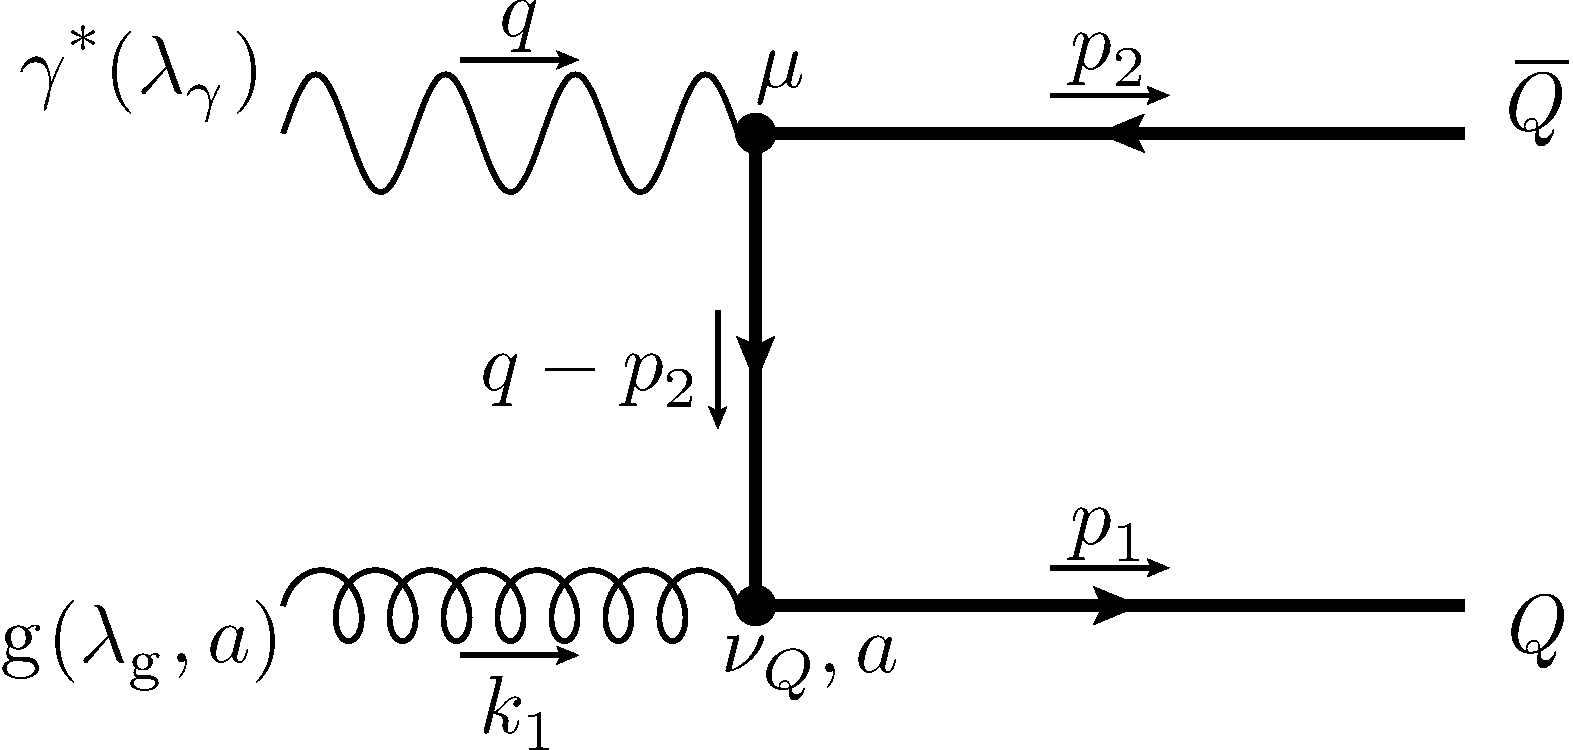
\includegraphics[width=\textwidth]{pyfeyn/lo-a}
		\caption{$i\Md^{(LO)}_{1,\mu}$}
	\end{subfigure}\hspace{.15\textwidth}%
	\begin{subfigure}[t]{.4\textwidth}
		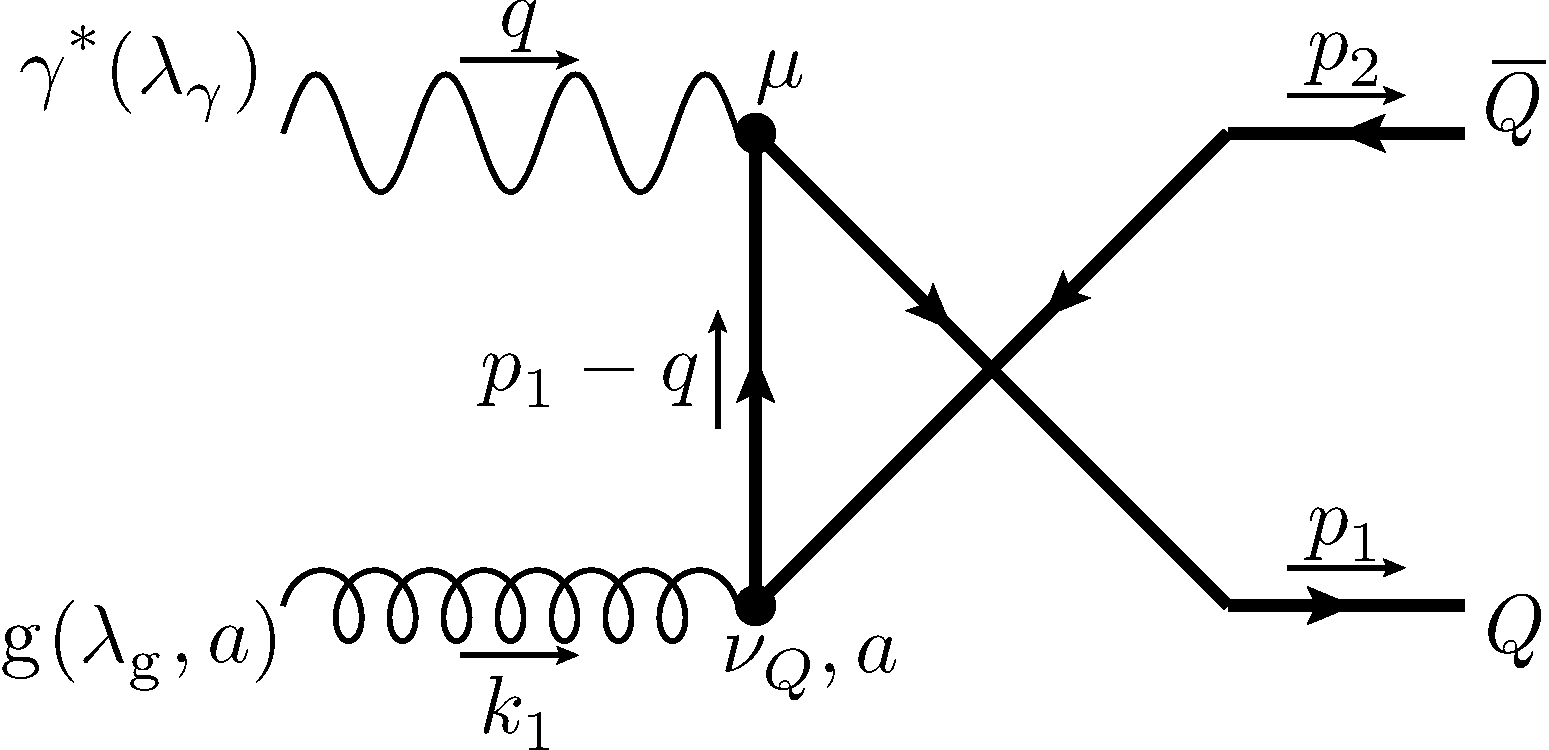
\includegraphics[width=\textwidth]{pyfeyn/lo-b}
		\caption{$i\Md^{(LO)}_{2,\mu}$}
	\end{subfigure}
	\caption{LO contributions}\label{fig:FeynLO}
\end{figure}

formula:
\begin{align}
i\Md^{(LO)}_{1,\mu} &= \bar u(p_1)(igT_a\gamma^{\nu_Q})\frac{i(\slashed{q}-\slashed{p}_2+m)}{u_1}(-i e e_H \gamma_\mu)v(p_2)\varepsilon^{(\lambda_{\Pg})}_{\nu_Q}(k_1)\\
i\Md^{(LO)}_{2,\mu} &= \bar u(p_1)(-i e e_H \gamma_\mu)\frac{i(\slashed{p}_1-\slashed{q}+m)}{t_1}(igT_a\gamma^{\nu_Q})v(p_2)\varepsilon^{(\lambda_{\Pg})}_{\nu_Q}(k_1)
\end{align}

color space:
\begin{equation}
\abs{\Md^{(LO)}_{1,\mu}+\Md^{(LO)}_{2,\mu}}^2 \sim \tr(T_a T_a) = N_c C_F
\end{equation}

%resulting in:
%\begin{align}
%B_{G,QED} &=\\
%B_{L,QED} &=  -\frac{4q^2(st_1u_1-m^2(t_1+u_1)^2)}{{s'}^2t_1u_1}\\
%\Delta B_{QED} &= \frac 1 {s' t_1^2u_1^2}\left(-2 {m^2} {s'} ({t_1}^3 + {t_1}^2 {u_1} + {t_1} {u_1}^2 + {u_1}^3)+\right.\nonumber\\
% &\left. {t_1} {u_1} ({s'}^2 ({t_1} + {u_1}) + ({t_1} - {u_1})^2 ({t_1} + {u_1}) + {s'} ({t_1}^2 + {u_1}^2) + 
%    {q^2} (-({t_1} - {u_1})^2 + {s'} ({t_1} + {u_1})))\right)
%\end{align}
%in accordance with \cite{Laenen1993162} and \cite{Marco}\fxerror{insert}
